
%
% foundations - clustering
%

\section{Clustering}

Clustering is the task of grouping unlabeled data in an automated way. It can also be described as the unsupervised classification of patterns into groups. The techniques of cluster analysis are applied in numerous scenarios including data mining, document retrieval, image segmentation and pattern classification. They are used to solve different tasks including pattern-analysis, grouping, decision-making or machine-learning.

Cluster analysis has been studied since the early beginnings of computer science and applies to a broad number of research fields. Different research communities have created a variety of vocabularies to describe methods related to clustering. Analog to the term cluster analysis, other names are used in literature: Q-analysis, topology, grouping, comping, classification, numerical taxonomy and unsupervised pattern recognition.

As indicated, clustering is a wide and generic term. Often it is used to refer to specific concepts which are appropriate for solving specific tasks. This means that efficient clustering algorithms have been developed and studied over the years for certain research fields. While such algorithms might perform well under certain circumstances, they might be completely inappropriate for other use cases. Imagine, an algorithm that  fits image segmentation well but is less useful in machine-learning~\cite{Meert06clustermaps, Jain99clusterreview}.

Clustering is a general concept that applies to multivariate data. Spatial data in this sense is a special case, and 2-dimensional spatial data reduces the problem space even further to planar space. Figure~\ref{fig:clusters} visualizes such an example of clusters of point patterns in two dimensional space. Humans can understand and perform this kind of clustering tasks competitively whereas clustering in high-dimensional space is difficult for humans to obtain. 

\begin{figure}[h]
  \begin{center}
    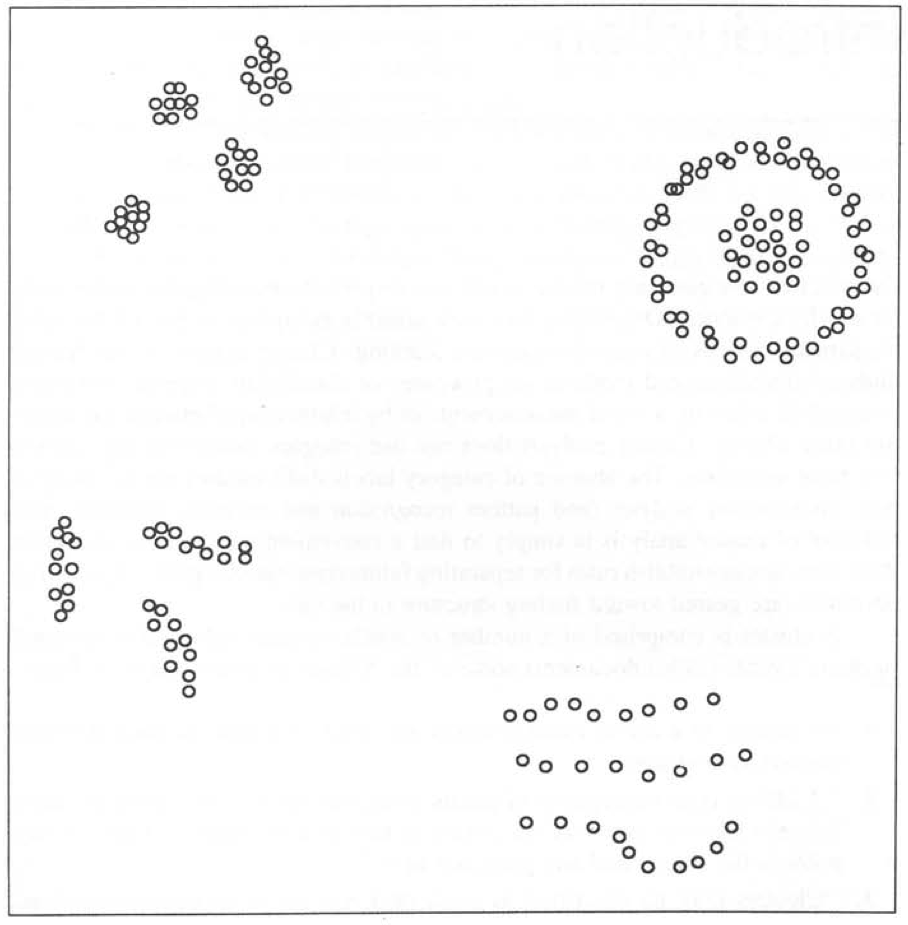
\includegraphics[width=0.75\textwidth]{figures/clusters.png}
    \caption{Clusters of point patterns in two dimensions~\cite[p 2]{Jain99clusterreview}.}
    \label{fig:clusters}
  \end{center}
\end{figure}



\subsection{The Clustering task}

Clustering is the task of aggregating items (also described as features) into clusters, based on similarities or proximity. A.K. Jain, M.N. Murty and P.J. Flynn~\cite{Jain99clusterreview} define the following steps involved in a typical pattern clustering activity:
 
\begin{quote}
\begin{enumerate}
\item pattern representation (optionally including feature extraction and/or selection), 
\item definition of a pattern proximity measure appropriate to the data domain, 
\item clustering or grouping, 
\item data abstraction (if needed), and 
\item assessment of output (if needed). 
\end{enumerate}
\end{quote}



\subsection{History}

K-means, one of the oldest and most widely used clustering algorithm was introduced already in 1967~\cite{MacQueen67kmeans, Meert06clustermaps}. Tryon and Bailey (1970) wrote one of the first books on cluster analysis. In 1973, Anderberg published ``Cluster analysis for applications'', a book that Jain and Dubes describe as ``the most comprehensive book for those who want to use cluster analysis''~\cite{Jain88clustering}.  While Tryon and Bailey focus on a single clustering approach (BC TRY), Anderberg already gives a comprehensive overview of clustering methods, strategies and a comparative evaluation of cluster analysis methods.

Clustering algorithms were improved and developed further over time, i.e. to account for performance issues. Prominent algorithms in that area include CLARANS~\cite{Ng94CLARANS} and BIRCH~\cite{Zhang96BIRCH} - they have a time complexity linear in the number of patterns. A popular, density based clustering algorithm is DBSCAN~\cite{Ester96DBSCAN}. Jain and Dubes summarize hierarchical and partitional clustering approaches in ``Algorithms for Clustering Data'' (1988) with a special focus on applications in image processing. Numerous subsequent publications on cluster analysis are released continuously~\cite{Jain99clusterreview}. 



\subsection{Cluster types}

Clusters are groupings of similar objects. Different models of interpretations of clusters exist: most notably, they can be classified into different types of clusters:

\begin{itemize}

\item \textbf{Well-separated} clusters have the property that objects within a cluster are closer to each other than any object outside of the cluster. As the name suggests, this is only possible when the data contains natural clusters that are quite far from each other.

\item \textbf{Prototype-based} clusters are defined so that objects are closer to their cluster's prototype than to any other one. Prototypes of clusters are either centroids (the mean of all points for a cluster) for continuous data or medoids (the most central point within a cluster) for categorical data.

\item \textbf{Graph-based} clusters can be defined as \emph{connected components} within a graph. That is a group of objects (nodes) where the objects are connected to one another but disconnected from objects outside of the cluster.

\item \textbf{Density-based} clusters group objects within dense regions that are surrounded by a region of low density. Such a definition is often employed when noise is present or clusters are irregular~\cite{Meert06clustermaps}.

\end{itemize}

\begin{figure}[h]
  \begin{center}
    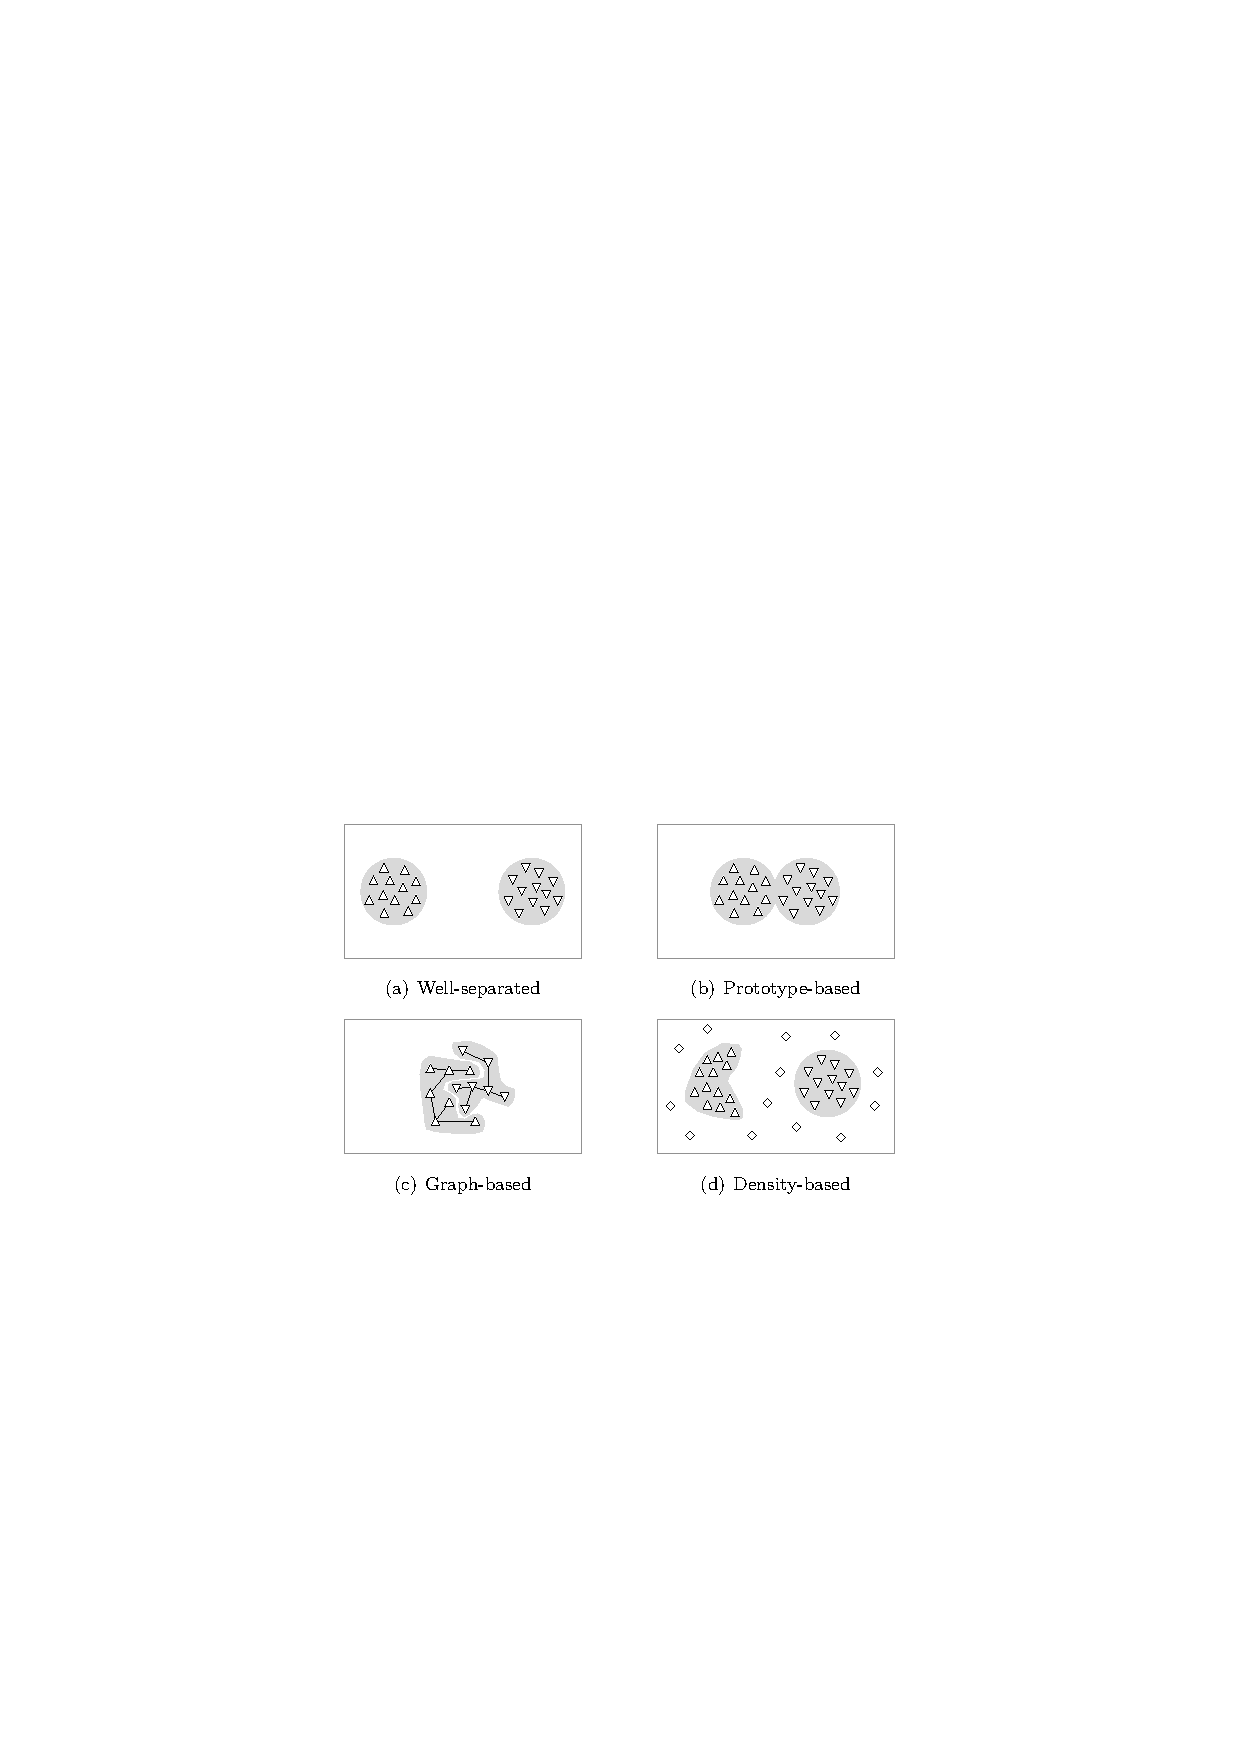
\includegraphics[width=0.75\textwidth]{figures/cluster_types.pdf}
    \caption{Types of clusters: (a) Well-separated, (b) Prototype-based, (c) Graph-based, (d) Density-based~\cite[p 9]{Meert06clustermaps}.}
    \label{fig:clusters}
  \end{center}
\end{figure}



\subsection{Clustering techniques}
\label{chapter:clustering-techniques}

Literature research reveals classifications of clustering techniques according to various aspects. Jain, Murty and Flynn primarily group the algorithms into hierarchical and partitional ones~\cite{Jain99clusterreview}. On the other hand, Stein and Busch split them into hierarchical, iterative, density-based and meta-search-controlled~\cite{Stein05density}. The differentiation of properties into groupings of clustering techniques and cross-cutting aspects is inconsistent among publications. This again shows the wide variety in which cluster analysis is being discussed and developed.

\begin{figure}[h]
  \begin{center}
    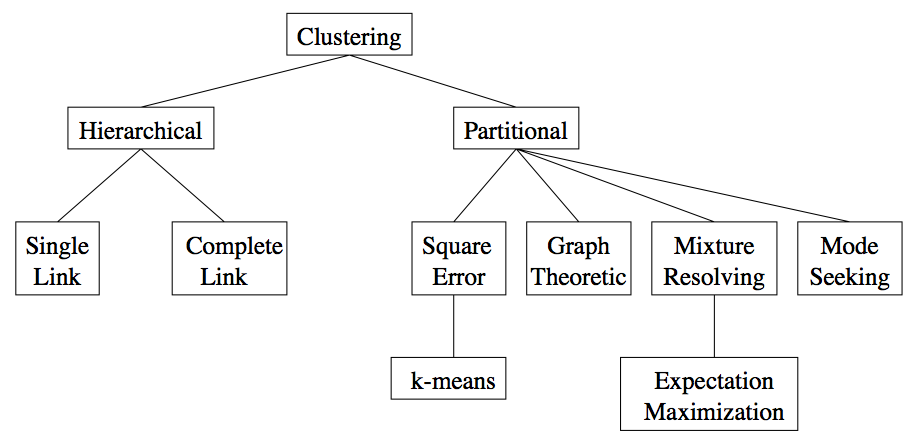
\includegraphics[width=0.9\textwidth]{figures/clustering_approaches_jain.png}
    \caption{A taxonomy of clustering approaches.~\cite[p 275]{Jain99clusterreview}.}
    \label{fig:clusters}
  \end{center}
\end{figure}

\begin{figure}[h]
  \begin{center}
    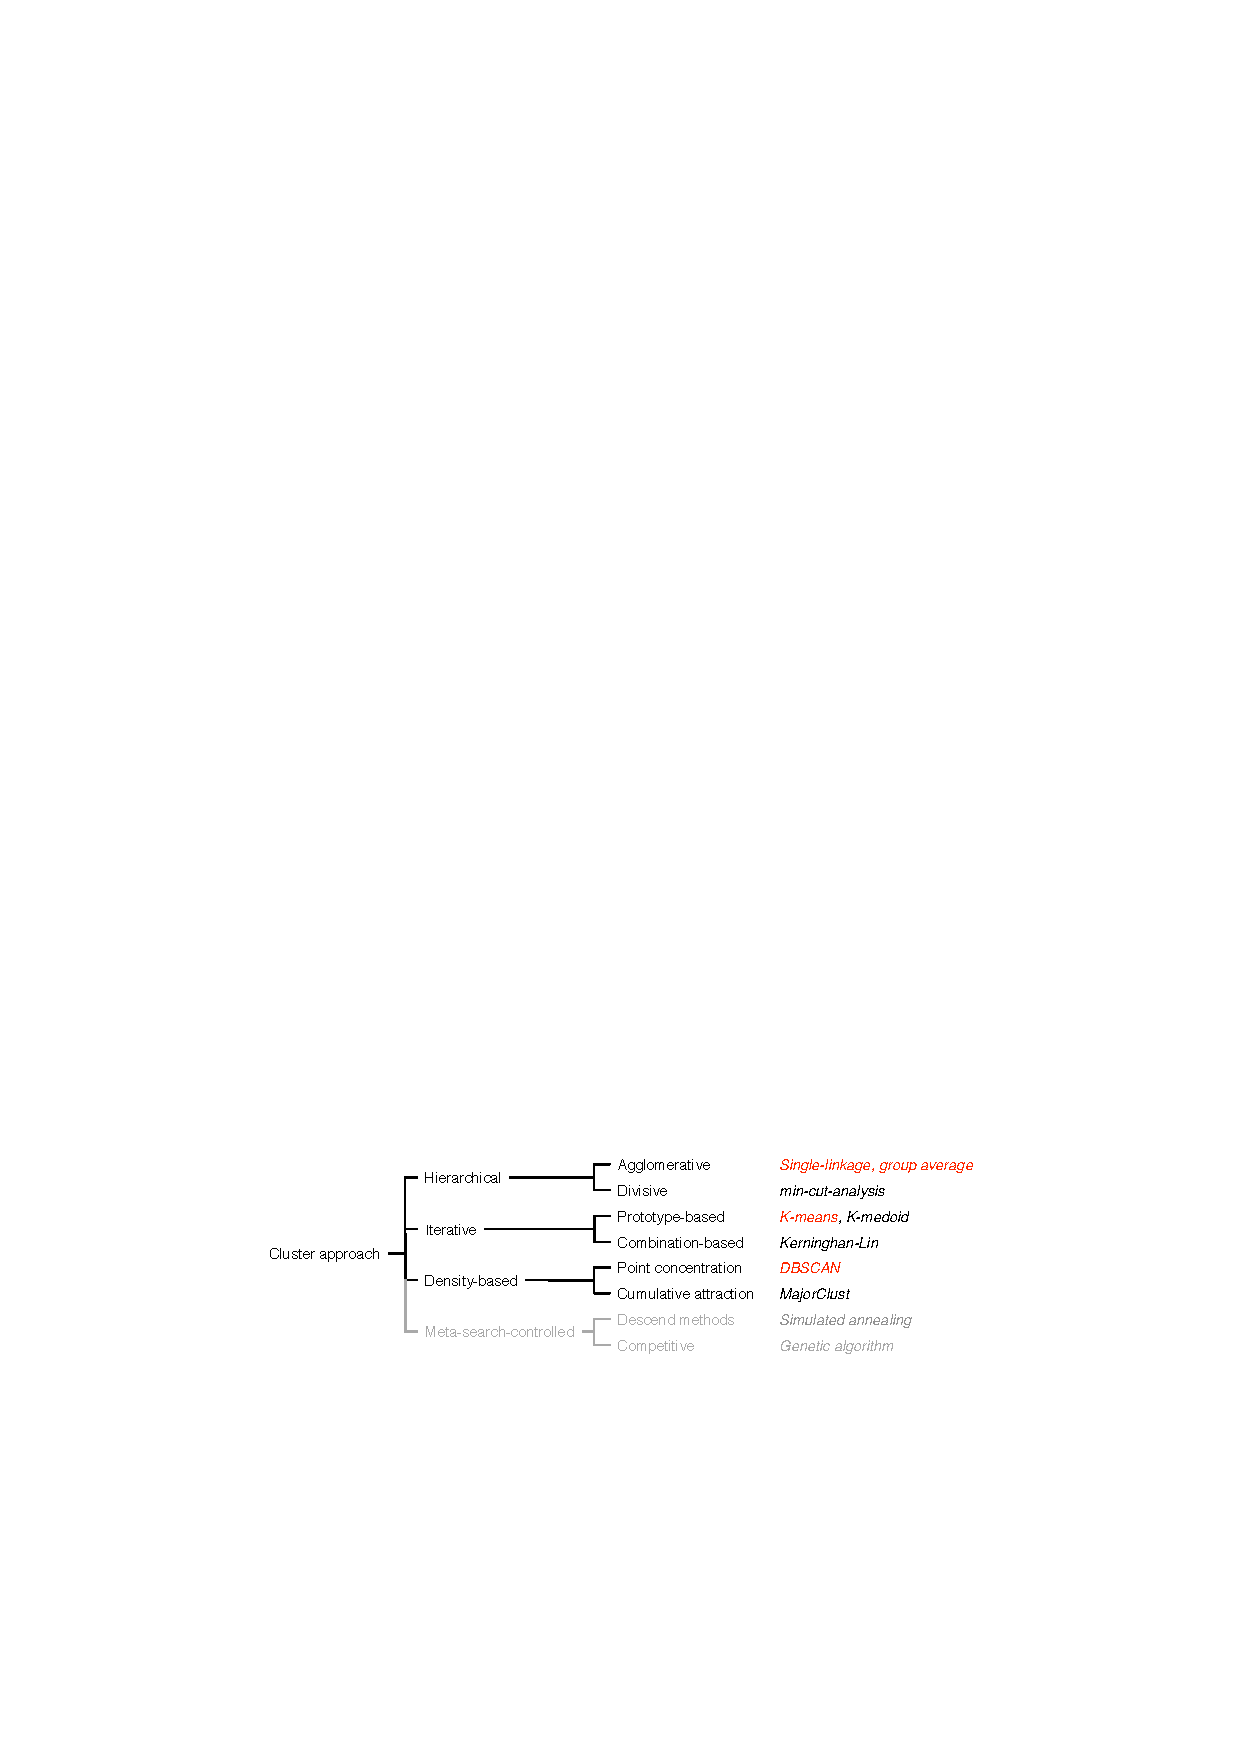
\includegraphics[width=1\textwidth]{figures/clustering_techniques_meert.pdf}
    \caption{A taxonomy of cluster algorithms as cited in~\cite[p 14]{Meert06clustermaps}, based on \cite{Stein05density}.}
    \label{fig:clusters}
  \end{center}
\end{figure}

\begin{itemize}

\item \textbf{Hierarchical versus Partitional}. Whether it is nested is the classic differentiation between clustering techniques. \textit{Partitional clustering} divides the data set into non-overlapping clusters. It usually is driven by an \textit{iterative} approach that optimized the result.
\textit{Hierarchical clustering} organizes clusters as a tree. Each node in the tree is the union of its children. Both clustering types are related: applying partitional clusterings in a sequence can lead to a hierarchical clustering and cutting the hierarchical tree at a particular level produces a partitional clustering~\cite{Meert06clustermaps}. 

An example of the relationship between hierarchical and partitional clustering is given by the following example of density-based algorithms. \textit{DBSCAN} produces simple data partitions and was further developed into \textit{OPTICS} which clusters data hierarchically~\cite{wiki:DBSCAN}.     

\item \textbf{Agglomerative versus divisive}. \textit{Agglomerative clustering} algorithms start with single items and successively merge them together into clusters. On the other hand, \textit{divisive clustering} algorithms begin with a single cluster that contains all items and splits it up until a stopping criterion is met. Each such merging or splitting procedure can be seen as one level in the hierarchical clustering tree~\cite{Jain99clusterreview}.

\item \textbf{Hard versus Fuzzy}. \textit{Hard clustering} algorithms assign every item to a single cluster, this means that the clustering is \textit{exclusive}. A \textit{fuzzy clustering} algorithm may attribute an item to multiple clusters in a \textit{non-exclusive way }by assigning degrees of membership. A fuzzy clustering may be converted into a hard clustering by assigning every data item to the cluster with the highest degree of membership~\cite{Jain99clusterreview, Meert06clustermaps}.

\item \textbf{Complete versus Partial}. With \textit{complete clustering}, assigning every point to a cluster is required. \textit{Partial clustering} relaxes this requirement so that not every point needs to be assigned to a cluster. This can be particularly useful when clustering data sets with outliers and noise. In such cases, the partial clustering can be used to focus on crowded areas~\cite{Jain99clusterreview}. 

\end{itemize}

Further aspects include monothetic versus polythetic and incremental versus non-incremental clustering techniques. 



\subsection{Proximity}
\label{chapter:proximity}

Similarity is fundamental to the definition of a cluster. In order to measure similarity, clustering algorithms evaluate their proximity. Continuous data requires different proximity measurements than categorical data.

For continuos data, the proximity between items is typically quantified by dissimilarity in terms of distance measures. The three main distance functions are visualized in figure~\ref{fig:clustering-proximity} and explained as follows\cite{Meert06clustermaps}:

\begin{figure}[h]
  \begin{center}
    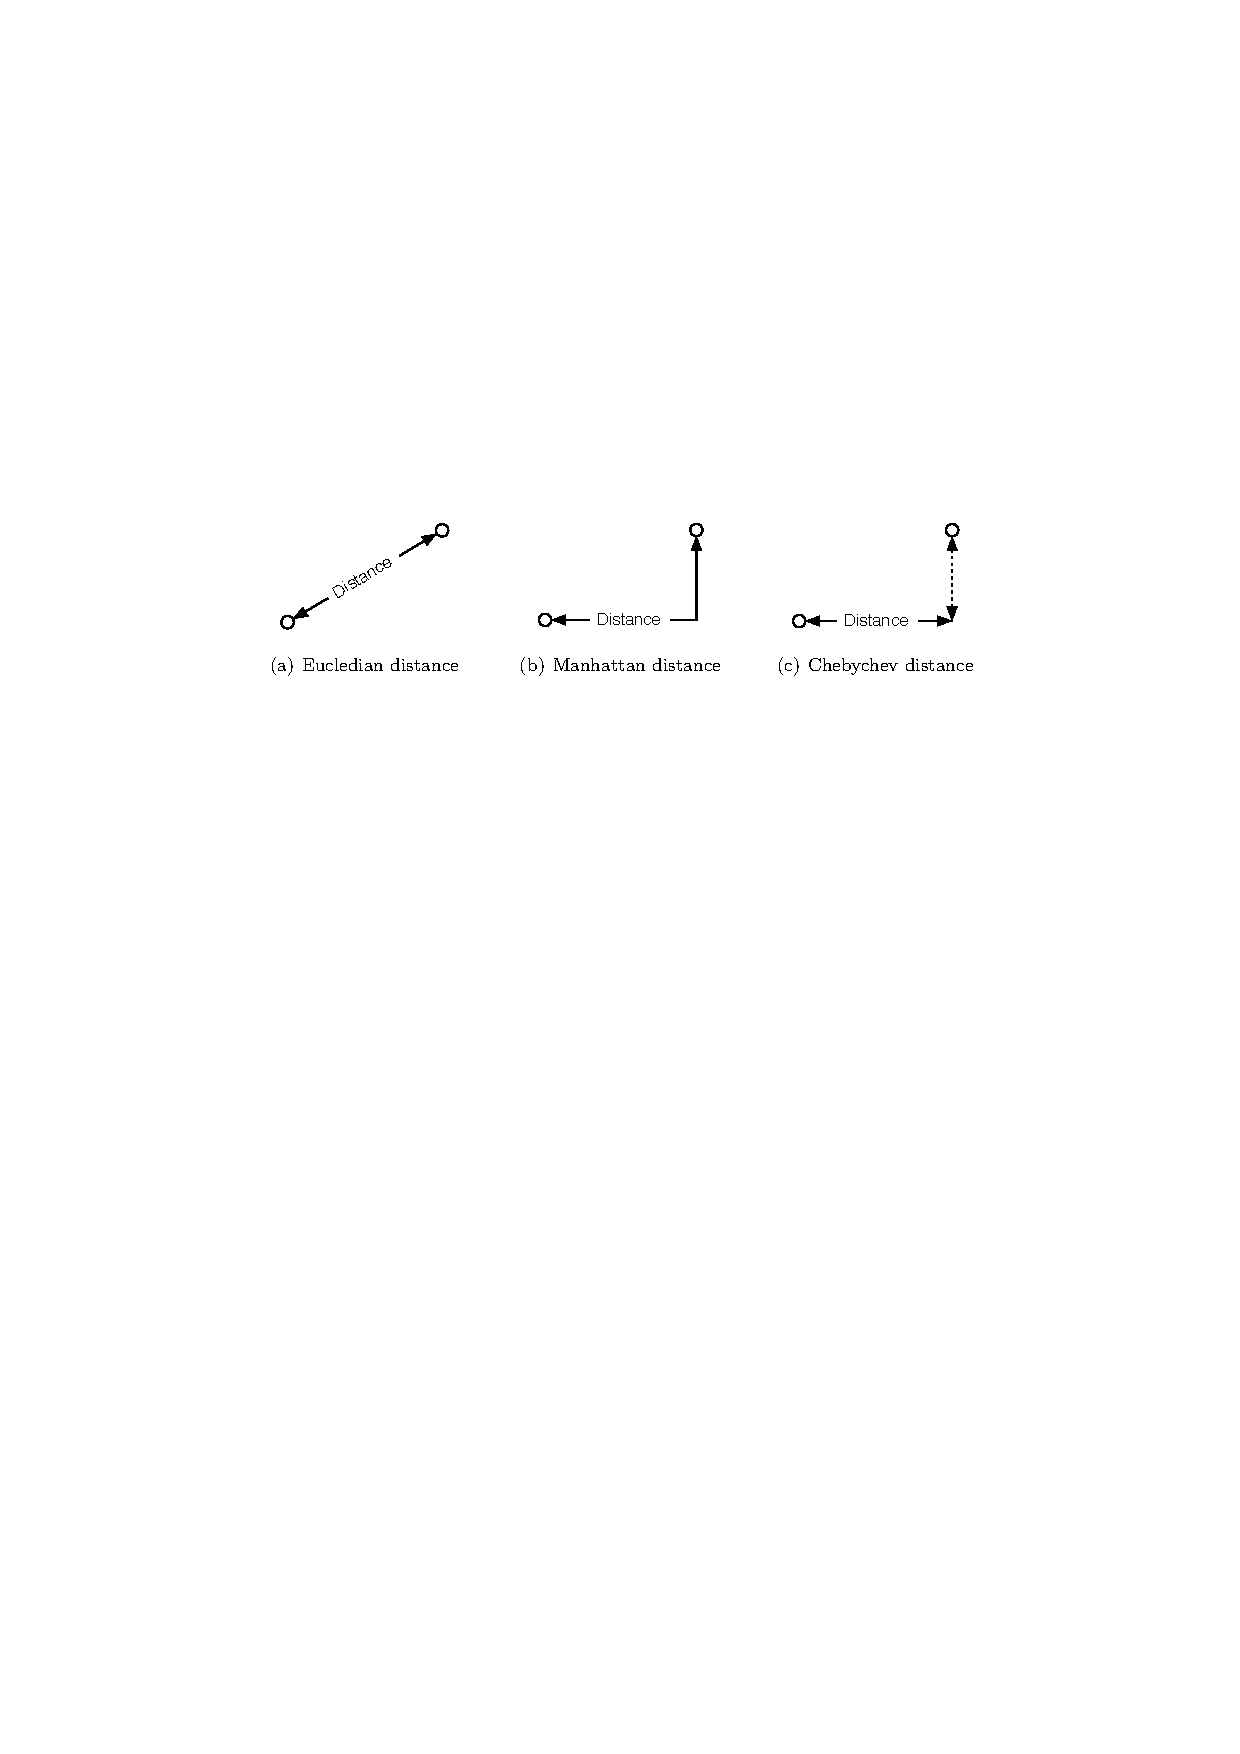
\includegraphics[width=1\textwidth]{figures/clustering_proximity.pdf}
    \caption{Distance measures for continuous data~\cite[p 12]{Meert06clustermaps}.}
    \label{fig:clustering-proximity}
  \end{center}
\end{figure}

\begin{itemize}

\item \textbf{Euclidian distance}. The euclidian distance is the geometric distance in the n-dimensional space. It is is the most common type of distance and defined as
\[ distance(x, y) = \sqrt{\sum_{i} (x_i - y_i)^2} \]

\item \textbf{Manhattan distance}. The manhattan distance, also known as city-block distance is distance when walking from one point to another following the axes. Compare with walking by following a raster like in manhattan. It is defined as
\[ distance(x, y) = \sum_{i} |x_i - y_i| \]

\item \textbf{Chebychev distance}. This distance measure returns the maximum distance between two points on any dimensions. It may be appropriate where two items are defined as `different', if they are different on any one of the dimensions.
\[ distance(x, y) = max |x_i - y_i| \]

\end{itemize}


\subsection{Clustering algorithms}

Researchers have created a multitude of algorithms, each appropriate for a certain task. As we will find out later, the requirements to the spatial clustering algorithm for this thesis are specific, which out-rules most scientific clustering algorithms which are geared towards image recognition or other disciplines. To provide an overview and to understand the basic differentiation of clustering techniques explained in \ref{chapter:clustering-techniques}, in this chapter we will introduce 3 foundational clustering algorithms: \textit{K-means}, \textit{Agglomerative Hierarchical Clustering Algorithm} and \textit{DBSCAN}.

\begin{itemize}

\item \textbf{Squared Error Algorithms: K-means}. The K-means is the most commonly used and simple algorithm based on a \textit{squared error criterion}. It creates a one-level partitioning of the data items by dividing them into \textit{K} clusters. By starting with a random initial partition it iteratively reassigns the patterns to clusters based on similarity.  The clustering process is completed when a convergence criterion is met, i.e. no further reassignments happen. Clusters are defined by \textit{cluster prototypes}: the centroid of the clustered items. Alternatively, the \textit{K-medoid} algorithm uses the most representative data item instead of the centroid.

The time complexity of the K-means algorithm is linear to the number of points:
\[time~complexity = \BigO{n}\]

\begin{algorithm}[t]
  \SetKwInOut{Input}{input}
  \Input{the number of clusters, $K$}
  \BlankLine
  {Select $K$ points as initial centroids}\;
  \While{Centroids do change}{
    {Form $K$ clusters by assigning each point to its closest centroid}\;
    {Recompute the centroid of each cluster}\;
  }
  \caption{K-means algorithm~\cite{Meert06clustermaps}}
  \label{alg:k-means}
\end{algorithm}

The selection of initial centroids affects the final outcome of the clustering process. Choosing them randomly is a simple but not very affective approach which can be compensating by applying multiple runs of the algorithm to retrieve an optimal result set. Optimizations to the centroid initialization include applying a hierarchical clustering or choosing distant points in the beginning.

Assigning points to the closest centroid requires a proximity measure, as explained in \ref{chapter:proximity}. Simple measures like the Euclidian distance are preferred, as this step needs to happen repeatedly within the algorithm. For each cluster, the centroid needs to be recalculated afterwards. This procedure is repeated until centroids do not change any more \cite{Jain99clusterreview, Meert06clustermaps}.

Figure \ref{fig:clustering_k-means} illustrates a K-means clustering process.

\begin{figure}[h]
  \begin{center}
    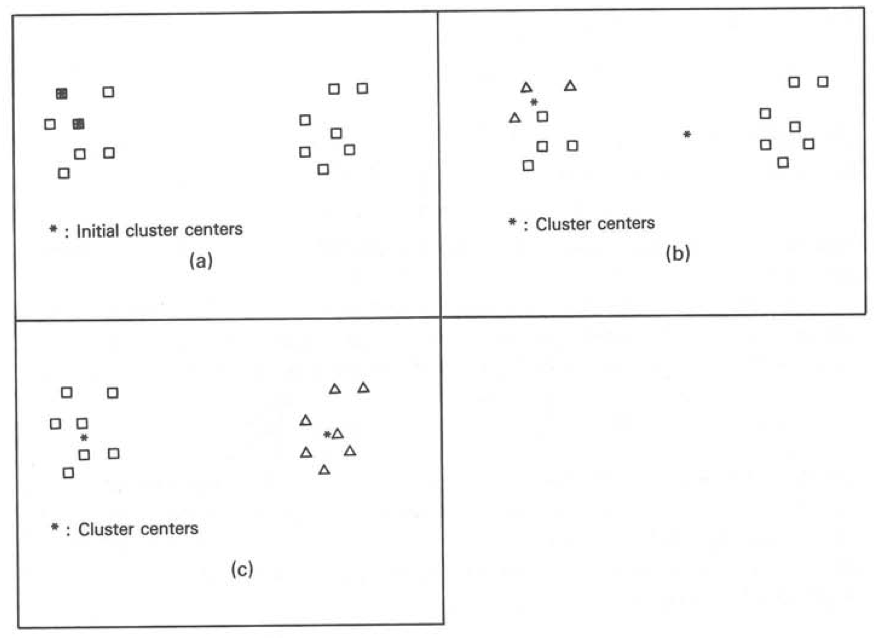
\includegraphics[width=0.9\textwidth]{figures/clustering_k-means.png}
    \caption{Convergence of K-means clustering: (a) initial data; (b) cluster membership after first loop; (c) cluster membership after second loop~\cite[p 99]{Jain88clustering}.}
    \label{fig:clustering_k-means}
  \end{center}
\end{figure}


\item \textbf{Agglomerative Hierarchical Clustering Algorithm}. This exemplary hierarchical clustering algorithm creates a hierarchy of nested sub clusters by serial partitioning. Its \textit{agglomerative} nature makes it start with every data item as a single clusters which get merged sub-sequentially. Alternatively, a \textit{divisive} hierarchical clustering would start with one cluster containing all data points and recursively split them up. At each level, a partitioning can be extracted, for example to serve as initial set of centroids for the previously discussed K-means algorithm. 

The time complexity of the agglomerative hierarchical clustering algorithm is:
\[time~complexity = \BigO{n^3}\]

\begin{algorithm}[t]
  {Assign each point to its individual cluster}\;
  {Compute the proximity matrix}\;
  \While{Number of clusters is larger than one}{
    {Merge the closest two clusters}\;
    {Update the proximity matrix to reflect the proximity between the new cluster and the original clusters}\;
  }
  \caption{Agglomerative hierarchic algorithm~\cite{Meert06clustermaps}}
  \label{alg:hierarchical}
\end{algorithm}

At the beginning of the agglomerative hierarchical clustering algorithm, each point is assigned to its own cluster. A proximity matrix is calculated that stores the distance of each pair of data item based on the chosen proximity measure.

To merge the two closest clusters, different heuristics may be applied. Most importantly, \textit{single-link} hierarchical clustering algorithms measure the distance between two clusters by the \textit{minimum} distance between all pairs of items from the two clusters. In contrast, \textit{complete-link} algorithms use the \textit{maximum} distance to create compact clusters and prevent chaining effects. Other approaches are based on \textit{average linkage} or \textit{Ward's method}. After merging the clusters, the proximity matrix will be updated so it reflects the current state of the clustering process. This procedure is repeated until all clusters have been merged, each step in the loop yields a level in the hierarchical clustering~\cite{Jain88clustering, Jain99clusterreview, Meert06clustermaps}.

Figure~\ref{fig:clustering-hierarchical-dendrogram} illustrates a Agglomerative Hierarchical clustering process as a dendrogram.

\begin{figure}[h]
  \begin{center}
    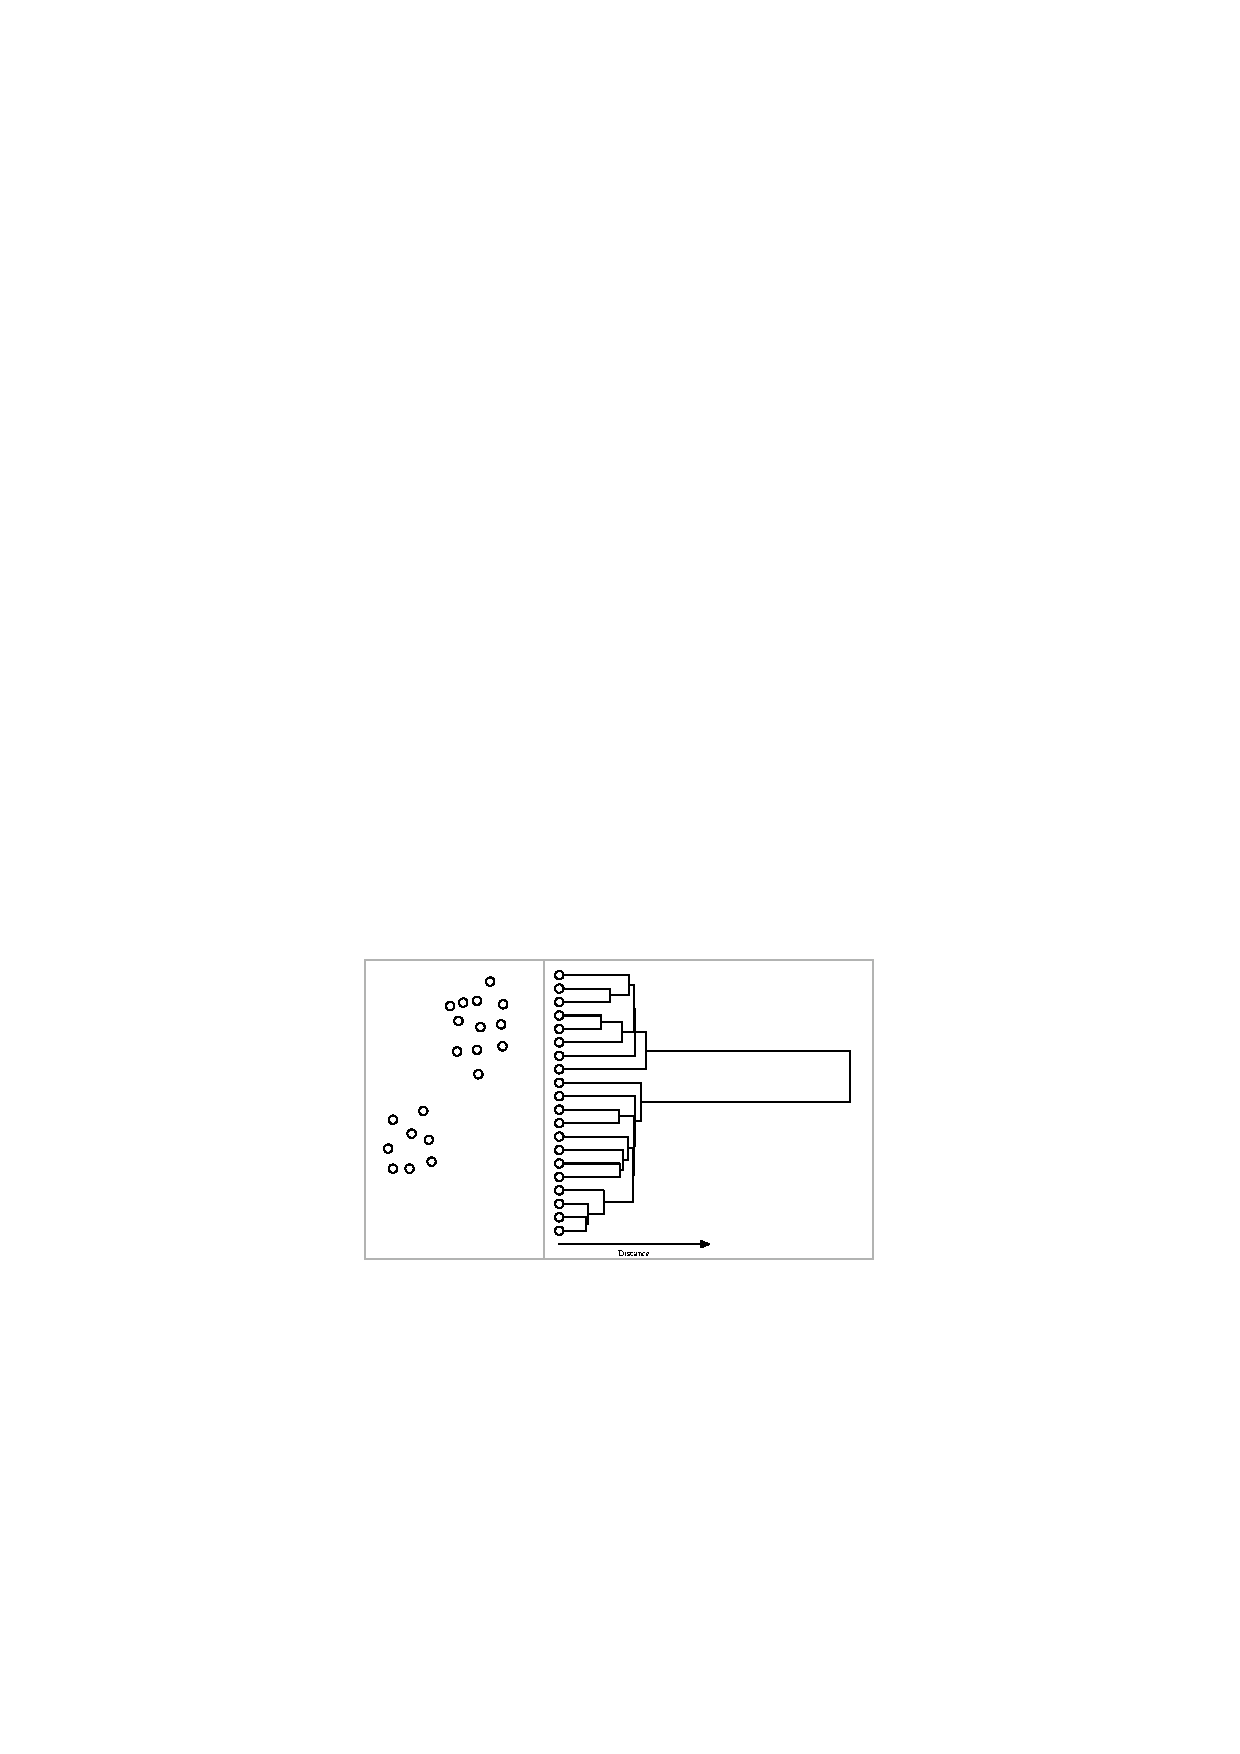
\includegraphics[width=0.9\textwidth]{figures/clustering_hierarchical_dendrogram.pdf}
    \caption{Dendrogram~\cite[p 20]{Meert06clustermaps}.}
    \label{fig:clustering-hierarchical-dendrogram}
  \end{center}
\end{figure}


\item \textbf{Density-based clustering algorithms: DBSCAN}. Density-based algorithms cluster regions of high density and separate them from regions with lower density. The density-based approach differentiates them from the previously discussed distance-based methods. This helps them overcome limitations of the former, as they tend to perform well in the detection of spherical-shaped clusters but perform weaker at discovering arbitrary shapes.
?
\begin{algorithm}[t]
  \While{Point is unclassified}{
    {Find points within region $\epsilon$}\;
    \If{number of points within region $> MinPts$} {
      {Start new cluster with Point}\;
      {Search regions of points in new cluster and expand cluster}\;
    }
  }
  \caption{DBSCAN algorithm~\cite{Meert06clustermaps}}
  \label{alg:dbscan}
\end{algorithm}

\textit{DBSCAN} takes a center-based approach, counting all points within a radius $\epsilon$. Based on density, it classifies points as \textit{core points} if the number of points within neighborhood exceeds a threshold defined as $MinPts$. \textit{Border points} don't match the previous criterion but fall into the neighborhood of a core point. Finally \textit{noise points} are outside of any neighborhood and therefore are neither core points nor border points \cite{Varlaro08spatial, Meert06clustermaps}. 

Figure~\ref{fig:clustering-dbscan} illustrates a DBSCAN clustering process.

\begin{figure}[h]
  \begin{center}
    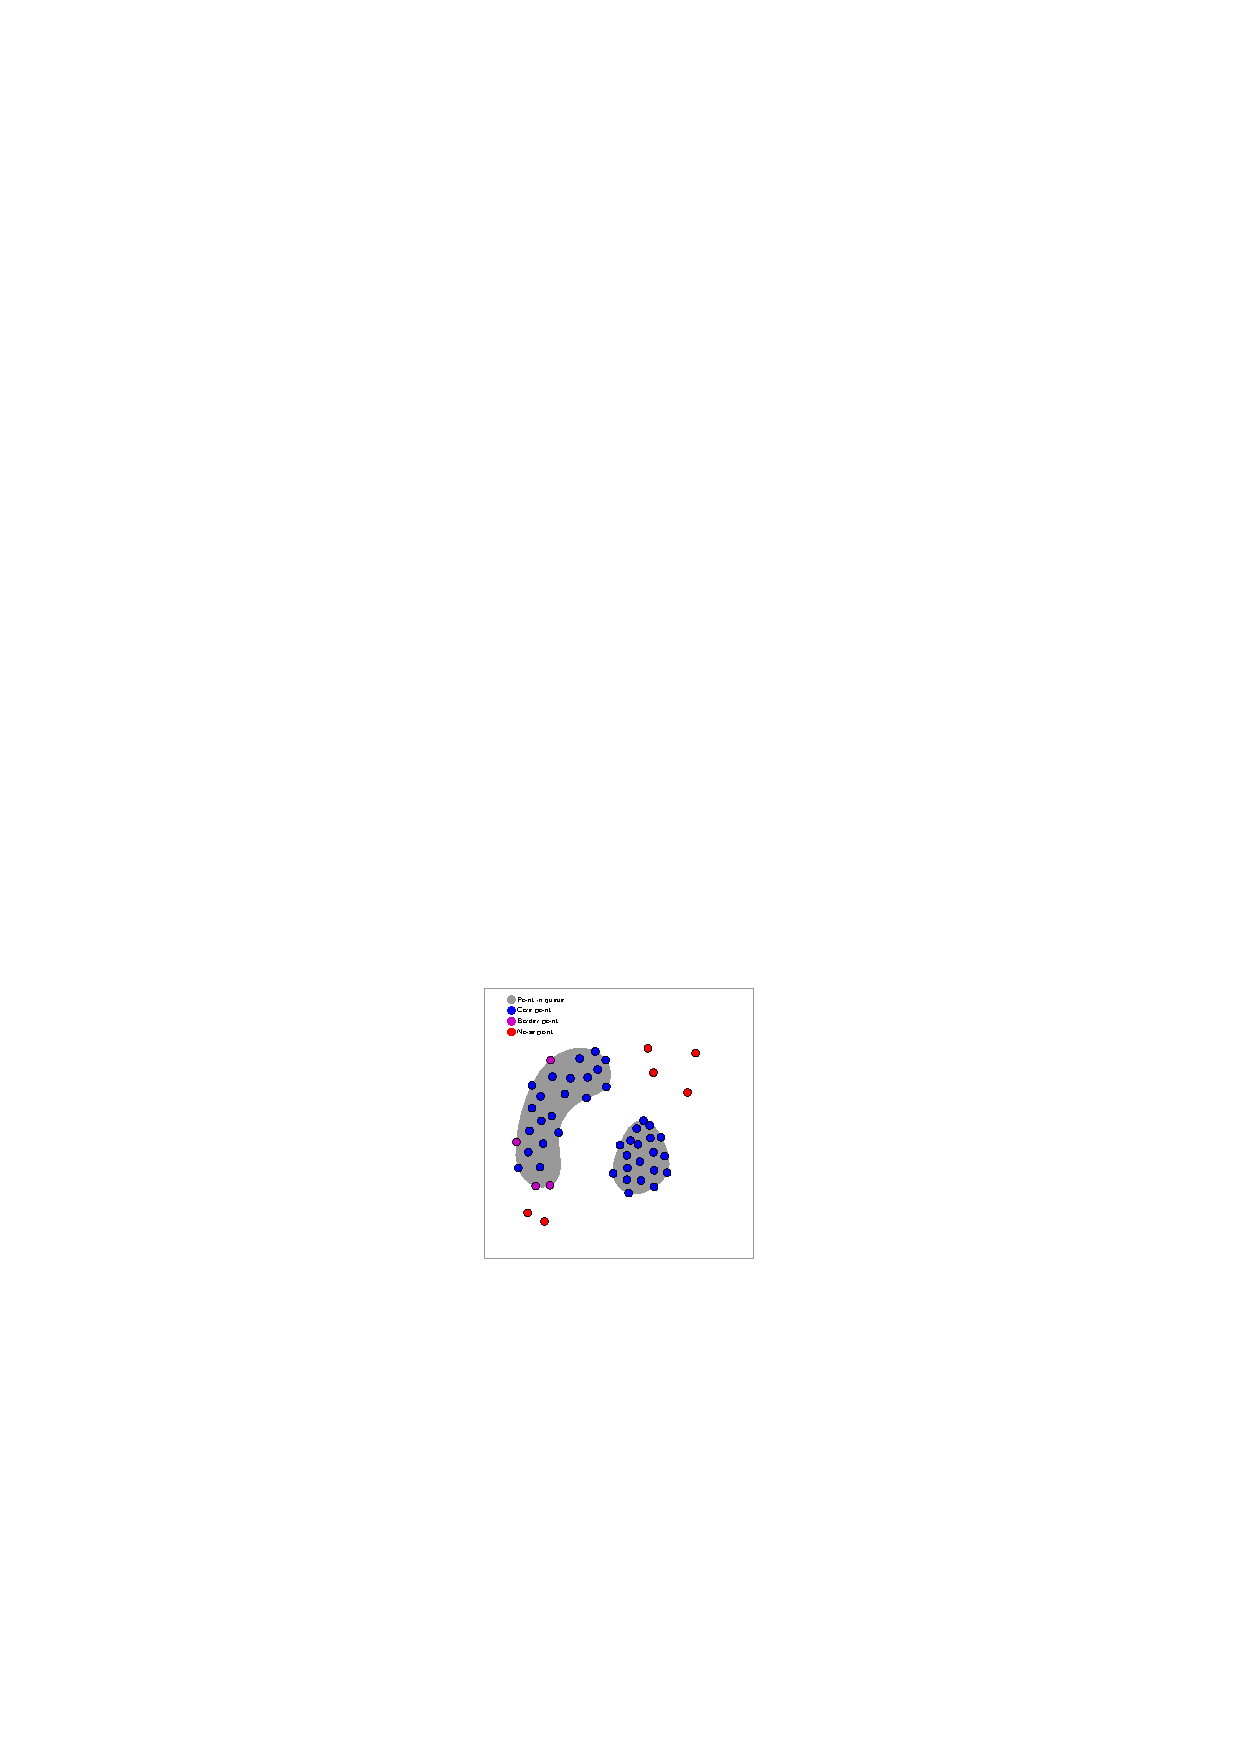
\includegraphics[width=0.55\textwidth]{figures/clustering_dbscan.pdf}
    \caption{DBSCAN algorithm~\cite[p 26]{Meert06clustermaps}.}
    \label{fig:clustering-dbscan}
  \end{center}
\end{figure}


\end{itemize}


























